\begin{ccRefFunctionObjectConcept}{Kernel::CompareY_2}
A model for this must provide:

\ccCreationVariable{fo}

\ccMemberFunction{Comparison_result operator()(const Kernel::Point_2&p, 
                                               const Kernel::Point_2&q);}
      {Compares the Cartesian $y$-coordinates of points \ccStyle{p} and
      \ccStyle{q}}

\begin{ccHtmlOnly}
<img border=0 src="fig/compare1.gif" align=middle alt="Comparison of the x 
or y coordinates of the (implicitly given) points in the boxes">
\end{ccHtmlOnly} 

\begin{ccTexOnly}
\begin{figure}[h]
\centerline{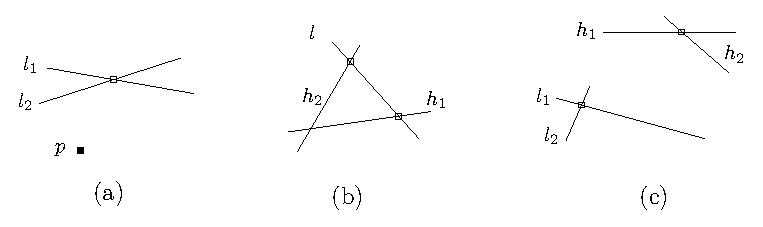
\includegraphics{Kernel_23_ref/fig/compare1}}
\caption{Comparison of the $x$ or $y$-coordinates of the (implicitly
given) points in the boxes.\label{fig-compare14}}
\end{figure} 
\end{ccTexOnly} 


\ccMemberFunction{Comparison_result operator()(const Kernel::Point_2 &p,
                                        const Kernel::Line_2 &l1,
                                        const Kernel::Line_2 &l2);}
        {compares the $y$-coordinates of $p$ and the 
         \ccHtmlNoLinksFrom{intersection} of lines
         $l1$ and $l2$%
         \ccTexHtml{ (Figure~\ref{fig-compare14} (a))}{, see (a) in the figure 
         above}.}


\ccMemberFunction{Comparison_result operator()(const Kernel::Line_2 &l,
                                        const Kernel::Line_2 &h1,
                                        const Kernel::Line_2 &h2);}
        {compares the $y$-coordinates of the \ccHtmlNoLinksFrom{intersection} of line $l$
         with line $h1$ and with line $h2$%
         \ccTexHtml{ (Figure~\ref{fig-compare14} (b))}{, see (b) in the figure 
         above}.}


\ccMemberFunction{Comparison_result operator()(const Kernel::Line_2 &l1,
                                        const Kernel::Line_2 &l2,
                                        const Kernel::Line_2 &h1,
                                        const Kernel::Line_2 &h2);}
        {compares the $y$-coordinates of the \ccHtmlNoLinksFrom{intersection} of lines $l1$
         and $l2$ and  the \ccHtmlNoLinksFrom{intersection} of lines $h1$ and $h2$ 
         \ccTexHtml{ (Figure~\ref{fig-compare14} (c))}{, see (c) in the figure 
         above}.}


\ccRefines
AdaptableFunctor (with two arguments)

\ccSeeAlso
\ccRefIdfierPage{CGAL::compare_y} \\

\end{ccRefFunctionObjectConcept}
